\documentclass{standalone}
\usepackage{tikz}
\usetikzlibrary{patterns, positioning}
\usepackage[sfdefault]{ClearSans} %% option 'sfdefault' activates Clear Sans as the default text font
\usepackage[T1]{fontenc}

\begin{document}
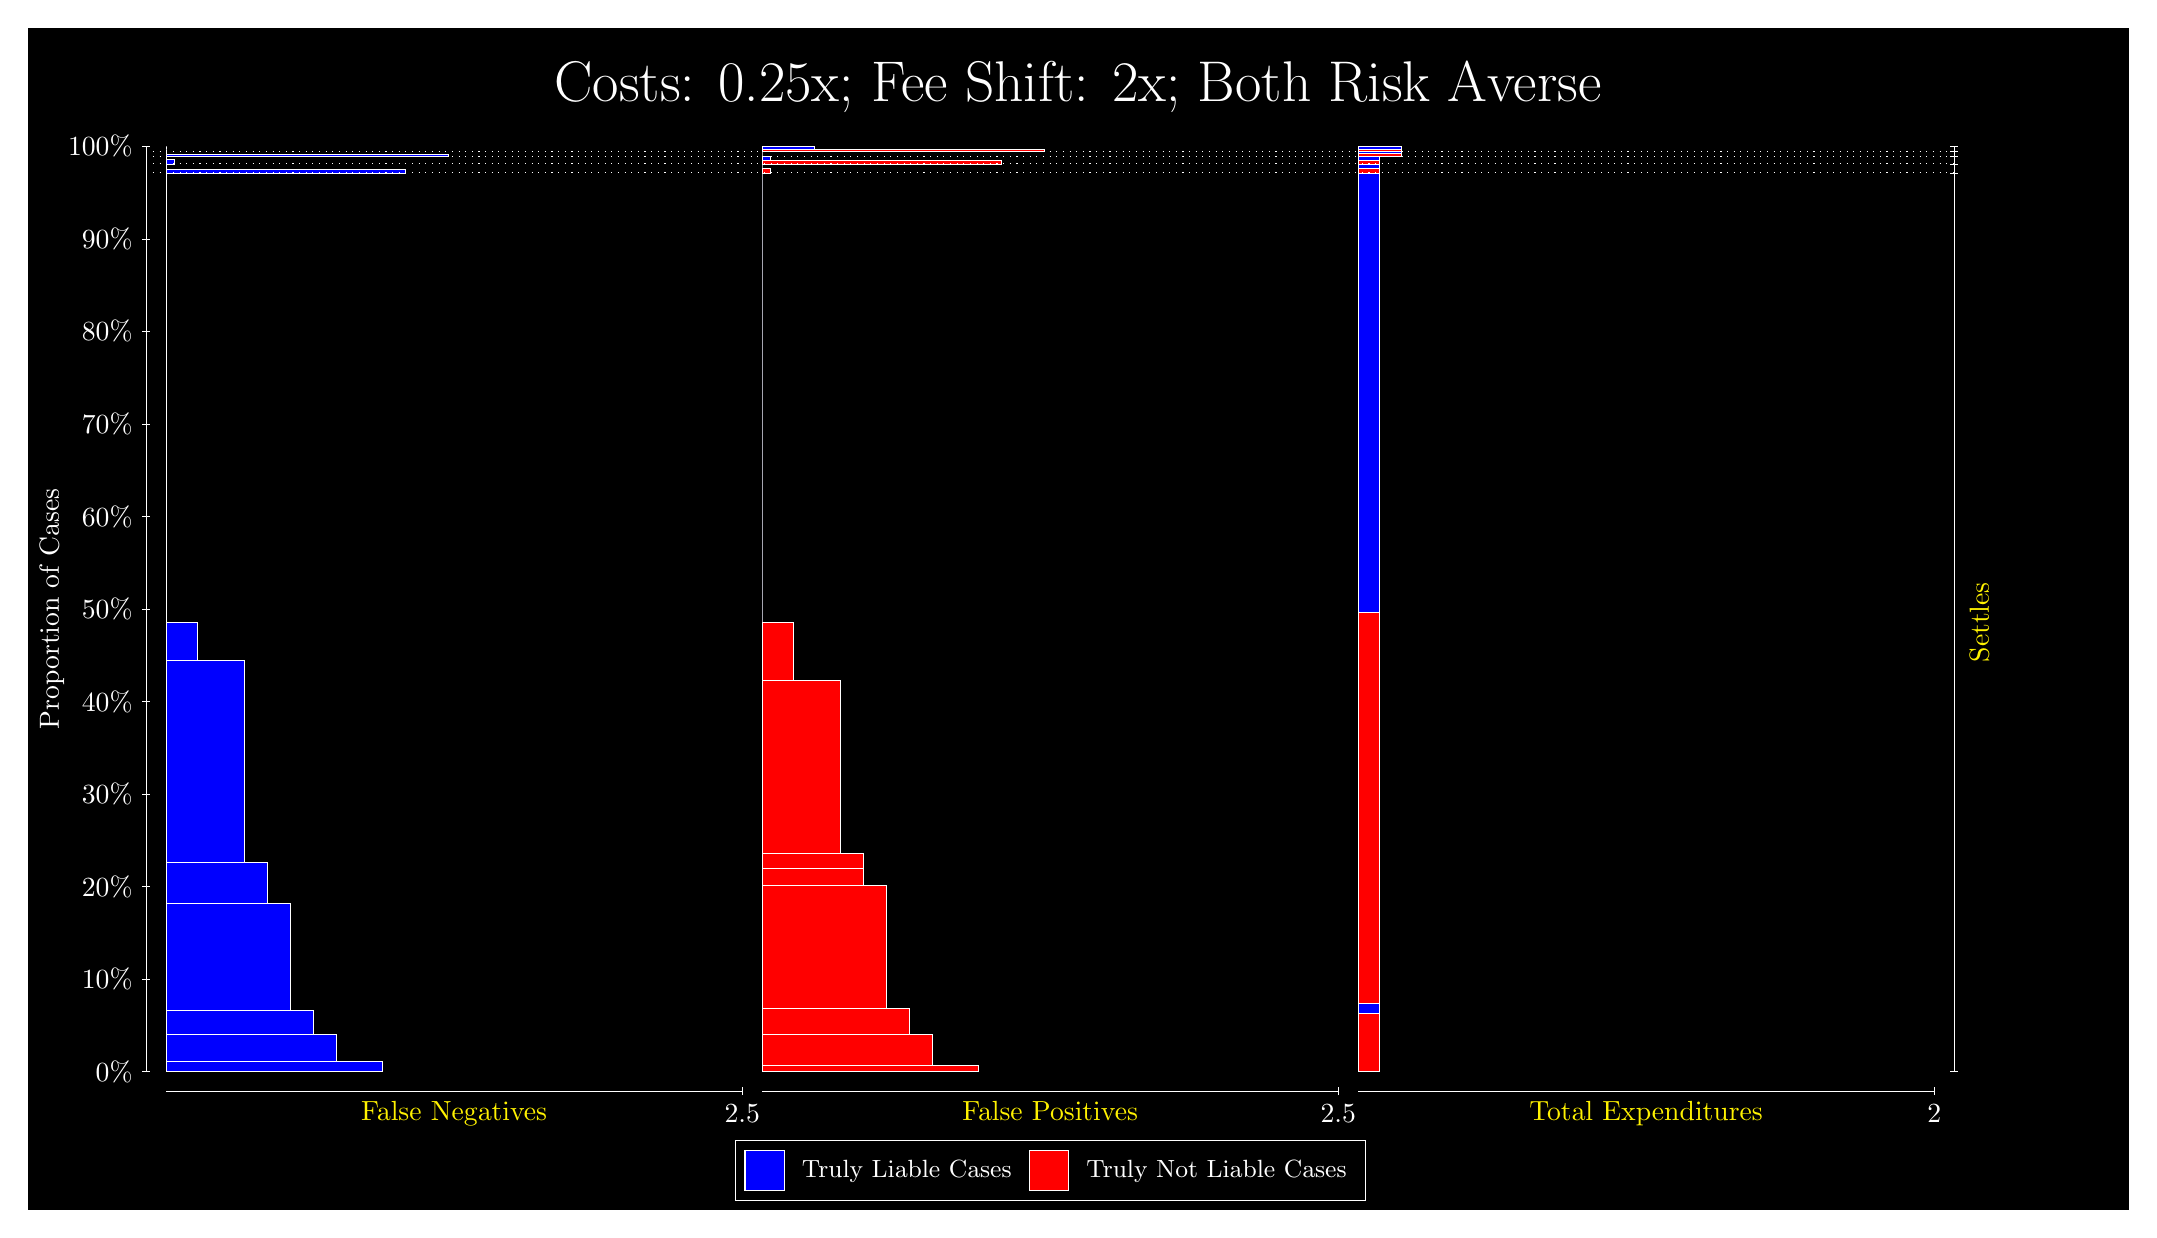
\begin{tikzpicture}
\draw[fill=black] (0,0) rectangle (26.667,15);
\draw[text=white] (0,13.5) rectangle (26.667,15) node[midway] {\huge Costs: 0.25x; Fee Shift: 2x; Both Risk Averse};
\draw[white, very thin] (1.5,1.75) -- (1.5,13.5);
\node[rotate=90, text=white, anchor=center] at (0.3, 7.625) {Proportion of Cases};
\draw[white, very thin] (1.45,1.75) -- (1.55,1.75);
\node[text=white, anchor=east] at (1.45, 1.75) {0\%};
\draw[white, very thin] (1.45,2.925) -- (1.55,2.925);
\node[text=white, anchor=east] at (1.45, 2.925) {10\%};
\draw[white, very thin] (1.45,4.1) -- (1.55,4.1);
\node[text=white, anchor=east] at (1.45, 4.1) {20\%};
\draw[white, very thin] (1.45,5.275) -- (1.55,5.275);
\node[text=white, anchor=east] at (1.45, 5.275) {30\%};
\draw[white, very thin] (1.45,6.45) -- (1.55,6.45);
\node[text=white, anchor=east] at (1.45, 6.45) {40\%};
\draw[white, very thin] (1.45,7.625) -- (1.55,7.625);
\node[text=white, anchor=east] at (1.45, 7.625) {50\%};
\draw[white, very thin] (1.45,8.8) -- (1.55,8.8);
\node[text=white, anchor=east] at (1.45, 8.8) {60\%};
\draw[white, very thin] (1.45,9.975) -- (1.55,9.975);
\node[text=white, anchor=east] at (1.45, 9.975) {70\%};
\draw[white, very thin] (1.45,11.15) -- (1.55,11.15);
\node[text=white, anchor=east] at (1.45, 11.15) {80\%};
\draw[white, very thin] (1.45,12.325) -- (1.55,12.325);
\node[text=white, anchor=east] at (1.45, 12.325) {90\%};
\draw[white, very thin] (1.45,13.5) -- (1.55,13.5);
\node[text=white, anchor=east] at (1.45, 13.5) {100\%};

\draw[white, very thin] (24.457,1.75) -- (24.457,13.5);
\draw[white, very thin] (24.407,1.75) -- (24.507,1.75);
\node[anchor=west] at (24.407, 1.75) {};
\draw[white, very thin] (24.407,13.163) -- (24.507,13.163);
\node[anchor=west] at (24.407, 13.163) {};
\draw[white, very thin] (24.407,13.278) -- (24.507,13.278);
\node[anchor=west] at (24.407, 13.278) {};
\draw[white, very thin] (24.407,13.376) -- (24.507,13.376);
\node[anchor=west] at (24.407, 13.376) {};
\draw[white, very thin] (24.407,13.436) -- (24.507,13.436);
\node[anchor=west] at (24.407, 13.436) {};
\draw[white, very thin] (24.407,13.5) -- (24.507,13.5);
\node[anchor=west] at (24.407, 13.5) {};

\draw[white, very thin, fill=blue] (1.75,1.75) rectangle (4.4946,1.8747);
\draw[white, very thin, fill=blue] (1.75,1.8747) rectangle (3.9091,2.2199);
\draw[white, very thin, fill=blue] (1.75,2.2199) rectangle (3.6163,2.5277);
\draw[white, very thin, fill=blue] (1.75,2.5277) rectangle (3.3236,3.8922);
\draw[white, very thin, fill=blue] (1.75,3.8922) rectangle (3.0308,4.4021);
\draw[white, very thin, fill=blue] (1.75,4.4021) rectangle (2.738,6.9739);
\draw[white, very thin, fill=blue] (1.75,6.9739) rectangle (2.1525,7.4522);
\draw[white, very thin, fill=red] (1.75,7.4522) rectangle (1.75,13.163);
\draw[white, very thin, fill=blue] (1.75,13.163) rectangle (4.7873,13.214);
\draw[white, very thin, fill=red] (1.75,13.214) rectangle (1.75,13.278);
\draw[white, very thin, fill=blue] (1.75,13.278) rectangle (1.8598,13.336);
\draw[white, very thin, fill=red] (1.75,13.336) rectangle (1.75,13.376);
\draw[white, very thin, fill=blue] (1.75,13.376) rectangle (5.3362,13.397);
\draw[white, very thin, fill=red] (1.75,13.397) rectangle (1.75,13.436);
\draw[white, very thin, fill=red] (1.75,13.436) rectangle (1.75,13.458);
\draw[white, very thin, fill=blue] (1.75,13.458) rectangle (1.75,13.5);
\draw[white, very thin, fill=red] (9.3189,1.75) rectangle (12.063,1.8249);
\draw[white, very thin, fill=red] (9.3189,1.8249) rectangle (11.478,2.223);
\draw[white, very thin, fill=red] (9.3189,2.223) rectangle (11.185,2.5559);
\draw[white, very thin, fill=red] (9.3189,2.5559) rectangle (10.892,4.1213);
\draw[white, very thin, fill=red] (9.3189,4.1213) rectangle (10.6,4.3292);
\draw[white, very thin, fill=red] (9.3189,4.3292) rectangle (10.6,4.5177);
\draw[white, very thin, fill=red] (9.3189,4.5177) rectangle (10.307,6.7157);
\draw[white, very thin, fill=red] (9.3189,6.7157) rectangle (9.7214,7.4603);
\draw[white, very thin, fill=blue] (9.3189,7.4603) rectangle (9.3189,13.163);
\draw[white, very thin, fill=red] (9.3189,13.163) rectangle (9.4287,13.227);
\draw[white, very thin, fill=blue] (9.3189,13.227) rectangle (9.3189,13.278);
\draw[white, very thin, fill=red] (9.3189,13.278) rectangle (12.356,13.318);
\draw[white, very thin, fill=blue] (9.3189,13.318) rectangle (9.4287,13.376);
\draw[white, very thin, fill=red] (9.3189,13.376) rectangle (9.3189,13.415);
\draw[white, very thin, fill=blue] (9.3189,13.415) rectangle (9.3189,13.436);
\draw[white, very thin, fill=red] (9.3189,13.436) rectangle (12.905,13.458);
\draw[white, very thin, fill=blue] (9.3189,13.458) rectangle (9.9776,13.5);
\draw[white, very thin, fill=red] (16.888,1.75) rectangle (17.162,2.4946);
\draw[white, very thin, fill=blue] (16.888,2.4946) rectangle (17.162,2.6193);
\draw[white, very thin, fill=red] (16.888,2.6193) rectangle (17.162,7.585);
\draw[white, very thin, fill=blue] (16.888,7.585) rectangle (17.162,13.163);
\draw[white, very thin, fill=red] (16.888,13.163) rectangle (17.162,13.227);
\draw[white, very thin, fill=blue] (16.888,13.227) rectangle (17.162,13.278);
\draw[white, very thin, fill=red] (16.888,13.278) rectangle (17.162,13.318);
\draw[white, very thin, fill=blue] (16.888,13.318) rectangle (17.162,13.376);
\draw[white, very thin, fill=red] (16.888,13.376) rectangle (17.437,13.415);
\draw[white, very thin, fill=blue] (16.888,13.415) rectangle (17.437,13.436);
\draw[white, very thin, fill=red] (16.888,13.436) rectangle (17.437,13.458);
\draw[white, very thin, fill=blue] (16.888,13.458) rectangle (17.437,13.5);
\draw[white, dotted] (1.5,13.163) -- (24.457,13.163);
\draw[white, dotted] (1.5,13.278) -- (24.457,13.278);
\draw[white, dotted] (1.5,13.376) -- (24.457,13.376);
\draw[white, dotted] (1.5,13.436) -- (24.457,13.436);
\draw[white, very thin] (1.75,1.5) -- (9.0689,1.5);
\node[text=yellow, anchor=north] at (5.4094, 1.5) {False Negatives};
\draw[white, very thin] (9.0689,1.45) -- (9.0689,1.55);
\node[text=white, anchor=north] at (9.0689, 1.45) {2.5};

\draw[white, very thin] (9.3189,1.5) -- (16.638,1.5);
\node[text=yellow, anchor=north] at (12.978, 1.5) {False Positives};
\draw[white, very thin] (16.638,1.45) -- (16.638,1.55);
\node[text=white, anchor=north] at (16.638, 1.45) {2.5};

\draw[white, very thin] (16.888,1.5) -- (24.207,1.5);
\node[text=yellow, anchor=north] at (20.547, 1.5) {Total Expenditures};
\draw[white, very thin] (24.207,1.45) -- (24.207,1.55);
\node[text=white, anchor=north] at (24.207, 1.45) {2};

\node[text=yellow, centered, rotate=90] at (24.777, 7.4563) {Settles};





\draw (12.978300999999998,1.5) node[draw=none] (baseCoordinate) {};
\begin{scope}[align=center]
        \matrix[scale=0.5, draw=white, below=0.5cm of baseCoordinate, nodes={draw}, column sep=0.1cm]{
            \node[rectangle, draw, minimum width=0.5cm, minimum height=0.5cm, fill=blue] {}; &
            \node[draw=none, font=\small, text=white] (B) {Truly Liable Cases}; &
            \node[rectangle, draw, minimum width=0.5cm, minimum height=0.5cm, fill=red] {}; &
            \node[draw=none, font=\small, text=white] (B) {Truly Not Liable Cases}; \\
            };
\end{scope}

\end{tikzpicture}
\end{document}